\usepackage{hyperref}\graphicspath{ {images/} }

\titledquestion{Attention exploration}[20]
\label{sec:analysis}

Multi-head self-attention is the core modeling component of Transformers.
In this question, we'll get some practice working with the self-attention equations, and motivate why multi-headed self-attention can be preferable to single-headed self-attention.

Recall that attention can be viewed as an operation on a \textit{query} vector $q\in\mathbb{R}^d$, a set of \textit{value} vectors $\{v_1,\dots,v_n\}, v_i\in\mathbb{R}^d$, and a set of \textit{key} vectors $\{k_1,\dots,k_n\}, k_i \in \mathbb{R}^d$, specified as follows:
\begin{align}
&c = \sum_{i=1}^{n} v_i \alpha_i \\
&\alpha_i = \frac{\exp(k_i^\top q)}{\sum_{j=1}^{n} \exp(k_j^\top q)}
\end{align} 
with $alpha = \{\alpha_1, \ldots, \alpha_n\}$ termed the ``attention weights''. 
Observe that the output $c\in\mathbb{R}^d$ is an average over the value vectors weighted with respect to $\alpha$.

\begin{parts}

\part[5] \textbf{Copying in attention.} One advantage of attention is that it's particularly easy to ``copy'' a value vector to the output $c$. In this problem, we'll motivate why this is the case.

\begin{subparts}
    \subpart[1] \textbf{Explain} why $\alpha$ can be interpreted as a categorical probability distribution. 
    
    \ifans{111Since it is the result of a softmax, it will result in a vector that sums to 1 and each value is greater than or equal to 0.}
    \subpart[2] The distribution $\alpha$ is typically relatively ``diffuse''; the probability mass is spread out between many different $\alpha_i$. However, this is not always the case. \textbf{Describe} (in one sentence) under what conditions the categorical distribution $\alpha$ puts almost all of its weight on some $\alpha_j$, where $j \in \{1, \ldots, n\}$ (i.e. $\alpha_j \gg \sum_{i \neq j} \alpha_i$). What must be true about the query $q$ and/or the keys $\{k_1,\dots,k_n\}$?
    
    \ifans{if the query $q$ is very close to to $k_j$ and distant from all other $k$'s.
    }
    \subpart[1] Under the conditions you gave in (ii),  \textbf{describe} the output $c$. 
    
    \ifans{$c$ will be close to $v_j$.}
    \subpart[1] \textbf{Explain} (in two sentences or fewer) what your answer to (ii) and (iii) means intuitively. \\
\ifans{that the query for the word is connected to a single word in the sentence only with high probability.}

\end{subparts}


\part[7]\textbf{An average of two.} 
\label{q_avg_of_two}
Instead of focusing on just one vector $v_j$, a Transformer model might want to incorporate information from \textit{multiple} source vectors. 
Consider the case where we instead want to incorporate information from \textbf{two} vectors $v_a$ and $v_b$, with corresponding key vectors $k_a$ and $k_b$.
\begin{subparts}
\subpart[3] How should we combine two $d$-dimensional vectors $v_a, v_b$ into one output vector $c$ in a way that preserves information from both vectors? 
In machine learning, one common way to do so is to take the average: $c = \frac{1}{2} (v_a + v_b)$.
It might seem hard to extract information about the original vectors $v_a$ and $v_b$ from the resulting $c$, but under certain conditions one can do so. In this problem, we'll see why this is the case.
\\ \\
Suppose that although we don't know $v_a$ or $v_b$, we do know that $v_a$ lies in a subspace $A$ formed by the $m$ basis vectors $\{a_1, a_2, \ldots, a_m\}$, while $v_b$ lies in a subspace $B$ formed by the $p$ basis vectors $\{b_1, b_2, \ldots, b_p\}.$ (This means that any $v_a$ can be expressed as a linear combination of its basis vectors, as can $v_b$. All basis vectors have norm 1 and are orthogonal to each other.)
Additionally, suppose that the two subspaces are orthogonal; i.e. $a_j^\top b_k = 0$ for all $j, k$.

Using the basis vectors $\{a_1, a_2, \ldots, a_m\}$, construct a matrix $M$ such that for arbitrary vectors $v_a \in A$ and $v_b \in B$, we can use $M$ to extract $v_a$ from the sum vector $s = v_a + v_b$. In other words, we want to construct $M$ such that for any $v_a, v_b$,  $Ms = v_a$. Show that $Ms = v_a$ holds for your $M$.


\textbf{Hint:} Given that the vectors $\{a_1, a_2, \ldots, a_m\}$ are both \textit{orthogonal} and \textit{form a basis} for $v_a$, we know that there exist some $c_1, c_2, \ldots, c_m$ such that $v_a = c_1 a_1 + c_2 a_2 + \cdots + c_m a_m$. Can you create a vector of these weights $c$? 

\ifans{We can set $M=AA^T$:
    \begin{align*}
        v_a &= Ac\\
        &= AIc\\
        &= A(A^TA)c\\
        &= AA^T(Ac)\\
        &= AA^T v_a\\
        &= AA^T v_a + A\pmb{0}\\
        &= AA^T v_a + A(A^T v_b)\\
        &= AA^T(v_a+v_b)\\
        &= AA^T s\\
        &= Ms
    \end{align*}
}

\subpart[4] As before, let $v_a$ and $v_b$ be two value vectors corresponding to key vectors $k_a$ and $k_b$, respectively.
Assume that (1) all key vectors are orthogonal, so $k_i^\top k_j = 0$ for all $i \neq j$; and (2) all key vectors have norm $1$.\footnote{Recall that a vector $x$ has norm 1 iff $x^\top x = 1$.}
\textbf{Find an expression} for a query vector $q$ such that $c \approx \frac{1}{2}(v_a + v_b)$, and justify your answer. \footnote{Hint: while the softmax function will never \textit{exactly} average the two vectors, you can get close by using a large scalar multiple in the expression.} 


\ifans{We need to have: $\alpha_i = \frac{1}{2}$, i.e., $k_a^T q = k_b^T q$. If we set $q=k_a+k_b$ we get:
\begin{equation*}
    k_a^T q = k_a^T k_a + k_a^T k_b = 1 + 0 = 1 = 0 + 1 = k_b^T k_a + k_b^T k_b = k_b^T q
\end{equation*}
}
\end{subparts}

\part[5]\textbf{Drawbacks of single-headed attention:} \label{q_problem_with_single_head}
In the previous part, we saw how it was \textit{possible} for a single-headed attention to focus equally on two values.
The same concept could easily be extended to any subset of values.
In this question we'll see why it's not a \textit{practical} solution.
Consider a set of key vectors $\{k_1,\dots,k_n\}$ that are now randomly sampled, $k_i\sim \mathcal{N}(\mu_i, \Sigma_i)$, where the means $\mu_i \in \mathbb{R}^d$ are known to you, but the covariances $\Sigma_i$ are unknown.
Further, assume that the means $\mu_i$ are all perpendicular; $\mu_i^\top \mu_j = 0$ if $i\not=j$, and unit norm, $\|\mu_i\|=1$.

\begin{subparts}
\subpart[2] Assume that the covariance matrices are $\Sigma_i = \alpha I, \forall i \in \{1, 2, \ldots, n\}$, for vanishingly small $\alpha$.
Design a query $q$ in terms of the $\mu_i$ such that as before, $c\approx \frac{1}{2}(v_a + v_b)$, and provide a brief argument as to why it works.

\ifans{}

\subpart[3] Though single-headed attention is resistant to small perturbations in the keys, some types of larger perturbations may pose a bigger issue. Specifically, in some cases, one key vector $k_a$ may be larger or smaller in norm than the others, while still pointing in the same direction as $\mu_a$. As an example, let us consider a covariance for item $a$ as $\Sigma_a = \alpha I + \frac{1}{2}(\mu_a\mu_a^\top)$ for vanishingly small $\alpha$ (as shown in figure \ref{ka_plausible}). This causes $k_a$ to point in roughly the same direction as $\mu_a$, but with large variances in magnitude. Further, let $\Sigma_i = \alpha I$ for all $i \neq a$. %
\begin{figure}[h]
\centering
\captionsetup{justification=centering,margin=2cm}
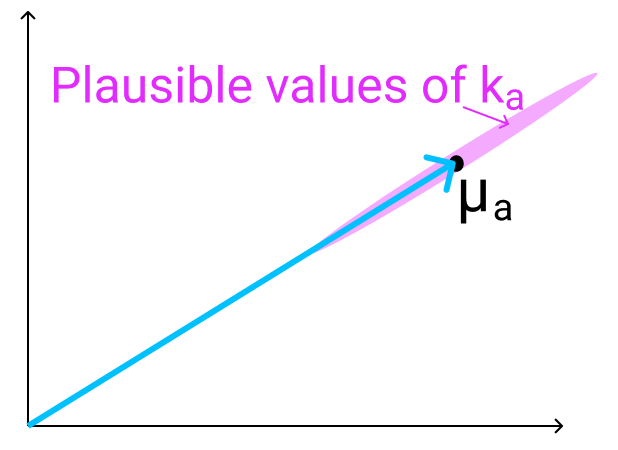
\includegraphics[width=0.35\linewidth]{images/ka_plausible.png}
\caption{The vector $\mu_a$ (shown here in 2D as an example), with the range of possible values of $k_a$ shown in red. As mentioned previously, $k_a$ points in roughly the same direction as $\mu_a$, but may have larger or smaller magnitude.}
\label{ka_plausible}
\end{figure}

When you sample $\{k_1,\dots,k_n\}$ multiple times, and use the $q$ vector that you defined in part i., what do you expect the vector $c$ will look like qualitatively for different samples? Think about how it differs from part (i) and how $c$'s variance would be affected.

\ifans{}
\end{subparts}

\part[3] \textbf{Benefits of multi-headed attention:}
Now we'll see some of the power of multi-headed attention.
We'll consider a simple version of multi-headed attention which is identical to single-headed self-attention as we've presented it in this homework, except two query vectors ($q_1$ and $q_2$) are defined, which leads to a pair of vectors ($c_1$ and $c_2$), each the output of single-headed attention given its respective query vector.
The final output of the multi-headed attention is their average, $\frac{1}{2}(c_1+c_2)$.
As in question 1(\ref{q_problem_with_single_head}), consider a set of key vectors $\{k_1,\dots,k_n\}$ that are randomly sampled, $k_i\sim \mathcal{N}(\mu_i, \Sigma_i)$, where the means $\mu_i$ are known to you, but the covariances $\Sigma_i$ are unknown.
Also as before, assume that the means $\mu_i$ are mutually orthogonal; $\mu_i^\top \mu_j = 0$ if $i\not=j$, and unit norm, $\|\mu_i\|=1$.
\begin{subparts}
\subpart[1]
Assume that the covariance matrices are $\Sigma_i=\alpha I$, for vanishingly small $\alpha$.
Design $q_1$ and $q_2$ such that $c$ is approximately equal to $\frac{1}{2}(v_a+v_b)$. 
Note that $q_1$ and $q_2$ should have different expressions.

\ifans{}

\subpart[2]
Assume that the covariance matrices are $\Sigma_a=\alpha I + \frac{1}{2}(\mu_a\mu_a^\top)$ for vanishingly small $\alpha$, and $\Sigma_i=\alpha I$  for all $i \neq a$.
Take the query vectors $q_1$ and $q_2$ that you designed in part i.
What, qualitatively, do you expect the output $c$ to look like across different samples of the key vectors? Explain briefly in terms of variance in $c_1$ and $c2$. You can ignore cases in which $k_a^\top q_i < 0$. 

\ifans{}



\end{subparts}







\end{parts}